% 31, 64, 92, 142
% unconstrained partial continuation ratio model, with hierarch structure

% why this is a sequential process --
% basic layout of sequential model
% we want to account for category specific effects
% and group level effects to account for repeats
% imputation
% likelihood and model layout
% fit via hamiltonian monte carlo in stan

\section*{Modeling sequential processes}


To model \emph{State- and Opposition-Focused ICC Transition} we need to account for the sequential way in which states and opposition actors transition through the ICC process (i.e., no ICC investigation, preliminary, and formal). Typically, scholars would use an ordinal regression framework to model such processes where what we are trying to model is the probability of falling at or below a given outcome category. Our dependent variables for state and opposition actors are grouped into three intervals -- 1 = no involvement; 2 = preliminary investigation; and 3 = formal investigation -- where the cumulative probability for category 2 is the probability that an actor is either in the no or preliminary investigation stage.\footnote{Stage models are also referred to as "continuation ratio" models \citep{fienberg:wasserman:1981, tutz1990sequential, agresti:2010} because the focus is on the sequential process of continuing from one stage to the next.} For an outcome with ($y$) with three categories (1-3), $y$ is linked to the binary outcomes in the cutpoint equations ($y_{1} - y_{2}$) by the measurement equations:

\begin{eqnarray}
	y_{1} =
	\begin{cases}
		1 \text{ if } y = 1 \nonumber \\
		0 \text{ if } y = 2-3 \nonumber \\
	\end{cases}
	y_{2} =
	\begin{cases}
		1 \text{ if } y = 1-2 \nonumber \\
		0 \text{ if } y = 3 \nonumber \\
	\end{cases}
\end{eqnarray}

In standard ordinal ordinal approaches, the sample size does not change across the cutpoint equations, specifically, every respondent is coded as 0 or 1 for the dependent variable in all of the cutpoint equations. The result of this is that the binary equations are no longer independent and thus can complicate our ability to draw inferences from statistical tests.\footnote{In the appendix, we compare the parameter estimates and performance of our approach with a standard ordinal framework. We show that not only do substantive results differ between the two approaches but that the ordinal framework is less accurate in terms of reflecting the data generating process underlying ICC investigations.}

The probability of interest in stage models is the conditional probability ($Pr[ y = k | y >= k]$), which is the probability for a particular category, $k$, given the respondent is in that category or a higher one. As a result, respondents in lower categories are excluded. The measurement equations in this case can be expressed as:

\begin{eqnarray}
	y_{1} =
	\begin{cases}
		1 \text{ if } y = 1 \nonumber \\
		0 \text{ if } y = 2-3 \nonumber \\
	\end{cases}
	y_{2} =
	\begin{cases}
		1 \text{ if } y = 2 | y >= 2 \nonumber \\
		0 \text{ if } y = 3 | y >= 2 \nonumber \\
	\end{cases}
\end{eqnarray}

The outcomes in the first cutpoint equation ($y_{1}$) is the same in the cumulative and stage models. However, the remaining cutpoint equations are different. In addition, the sample size becomes progressively smaller thus helping to ameliorate the issue of independence between the binary equations in later stages. To formalize the actual model, we follow \citet{tutz1990sequential} and \citet{agresti:2010} in utilizing a latent variable framework. For $y=1,\ldots,K$, there are $K-1$ latent variables. Each latent variable, $z_{m}$, corresponds to a particular cutpoint equation, for which the structural model can be expressed as:

\begin{align}
	z_{m} = x \beta + w\eta_{k}  + \epsilon_{k}
\end{align}

$x$ represents a vector of independent variables that are assumed to have a consistent effect, $\beta$, across stages and $w$ represent a vector of independent variables whose effect, captured by $\eta_{k}$, can vary by stage. $\epsilon_{k}$ represents the error term for the $k$ stage. Using this formulation we can represent the cutpoint equation for each stage as:

\begin{align}
	Pr(y = 1 | y >= 1, x, w) &= F(\tau_{1} - x\beta - w\eta_{1}) \\
	Pr(y = 2 | y >= 2, x, w) &= F(\tau_{2} - x\beta - w\eta_{2})
\end{align}

The sequential model assumes that for every category k -- stage of investigation at ICC -- there is a latent continuous variable $\tilde{Y_{k}}$ that determines the transition between the $k^{th}$ and the $k+1^{th}$ category. In our case, $\tilde{Y_{k}}$ represents all the factors contributing to the probability of a country proceeding beyond a given ICC investigation stage, $k$. Informally, we could call $\tilde{Y_{k}}$ ``suspicious level'' in the ongoing example. The categories are separated by thresholds $\tau_{k}$ -- perhaps thought of as the combination of all factors working against the country proceeding in ICC investigative stages. If $\tilde{Y_{k}}$ is greater than the threshold $\tau_{k}$, the sequential process continues; otherwise it stops at category $k$.

in order for actor $i$ to receive a value of $j$ for $Y_{i}$, the actor must pass through all levels less than $j$. The probability of then reaching $j$, conditional on the event that the $j^{th}$ level is reached, is given by:

\begin{eqnarray}
	Pr(y_{i}={j} | Y_{i} \geq {j}, \gamma, \beta) &=& F(\gamma_{j} - x_{i}^{'}\beta) \nonumber \\
	Pr(Y_{i}={j}|\gamma_{1},\beta) &=& F(\gamma_{j} - x_{i}^{'}\beta)\text{ }\prod^{j-1}_{k=1}\text{ }\{1-F(\gamma_{k}-x_{i}^{'}\beta)\} \nonumber
\end{eqnarray}

$\gamma = (\gamma_{1},...,\gamma_{J-1})$

\begin{eqnarray}
	Pr(y_{i}=J|\beta_{1},\gamma) &=&\text{}\prod^{J-1}_{k=1}\text{ }\{1-F(\gamma_{k}-x_{i}^{'}\beta)\} \nonumber
\end{eqnarray}

Latent variable representation

\begin{eqnarray}
	w_{ij} &=& x_{i}^{'}\beta+\epsilon_{ij},\text{ }\epsilon_{ij} \sim iid \nonumber
\end{eqnarray}

Observe:

\begin{eqnarray}
	y_{i} = 1\text{ iff } w_{i1} \leq \gamma_{1} \nonumber \\
	\nonumber \\
	y_{i} = 2\text{ iff }
	\begin{cases}
	w_{i1} > \gamma_{1} \nonumber \\
	w_{i2} \leq \gamma_{2} \nonumber \\
\end{cases}
\end{eqnarray}

Likelihood function:

\begin{eqnarray}
	L(\gamma,\beta) = \prod_{i\colon y_{i}<J}\text{ }[ F(\gamma_{y_{i}} - x_{i}^{'}\beta)\text{ }\prod_{k=1}^{y_{i}=1}\text{ }\{1-F(\gamma_{R}-x_{i}^{'}\beta)\}] &\times \displaystyle \prod_{i\colon y_{i}=J}\text{ }[\prod_{k=1}^{J=1} \{1-F(\gamma_{2} - x_{i}^{'}\beta)\}] \nonumber \\
	\nonumber \\
	(\gamma,\beta) \sim \pi (\gamma,\beta) & \nonumber \\
	\beta \sim N(\beta_{0},\Sigma_{0}) & \nonumber \\
	\nonumber \\
	z_{ij} = w_{ij} - \gamma_{j}, & \nonumber
	\end{eqnarray}
	So...
	\begin{eqnarray}
	y_{i} =
	\begin{cases}
	1\text{ if }z_{i} \leq 0 \nonumber \\
	2\text{ if }z_{i1} > 0, z_{i2} \leq 0 \nonumber \\
	\vdots \nonumber \\
	J-1\text{ if }z_{i1} > 0,...,z_{i,j-2}>0,z_{i,j-1}\leq0 \nonumber \\
	J\text{ if }z_{i1}>0,...,z_{i,j-1}>0
\end{cases}
\end{eqnarray}

Sample from the joint posterior of $(\{z_{ij}\},\beta)$

% Add note about how imputation process via semi parametric copula was embedded in the sampler:
% impute data via hollenbach et al. 2018/9 using semi parametric copula approach
% generates posterior distribution over missing data
%
% within the estimation process of teh sampler we pass in a randomly sampled missing dataset from posterior each time so that we can incorporate uncertainty from both missing data and estimation process

	% Hoff (2015) details a Bayesian implementation of this model via Gibbs sampling using semi-conjugate prior distributions to simulate parameter values from the posterior. We modify the sampler with respect to its accommodation of missing data. Specifically, we embed a semiparametric copula imputation scheme within the sampler such that at each iteration of the MCMC sampler for the regression a randomly sampled imputed dataset is supplied. The imputation scheme is described in more detail in Hollenbach et al. (2018), but for our purposes the main reason for including it within the sampler is so that the resulting parameters from the regression MCMC take into account both uncertainty within the model and the imputation process itself.

brief note on incorporation of random effects to deal with country-case heterogeneity

\begin{eqnarray}
	(\{z_{ij}\} | y,\beta)\text{ and }(\beta,|\{z_{ij}\},y) \nonumber \\
	(\{z_{ij}\} | y,\beta)\stackrel{iid}{\sim}TN_{(a,b)}(\beta,1) \nonumber \\
	\nonumber \\
	(\beta | \{z_{ij}\},y)\stackrel{iid}{\sim}N(\hat{\beta},\hat{\Sigma}) \nonumber \\
	\nonumber \\
	\hat{\beta} = (\Sigma_{0}^{-1}+\sum_{i=1}^{n} x_{i}^{'}x_{i})^{-1} \times (\Sigma_{0}^{-1}\beta_{0}+\sum_{i=1}^{n} x_{i}^{'}z_{i}) \nonumber \\
	\hat{\Sigma} = (\Sigma_{0}^{-1} + \sum_{i=1}^{n} x_{i}^{'}x_{i})^{-1} \nonumber
\end{eqnarray}


\section*{Empirical Results}

\begin{figure}
    \centering
    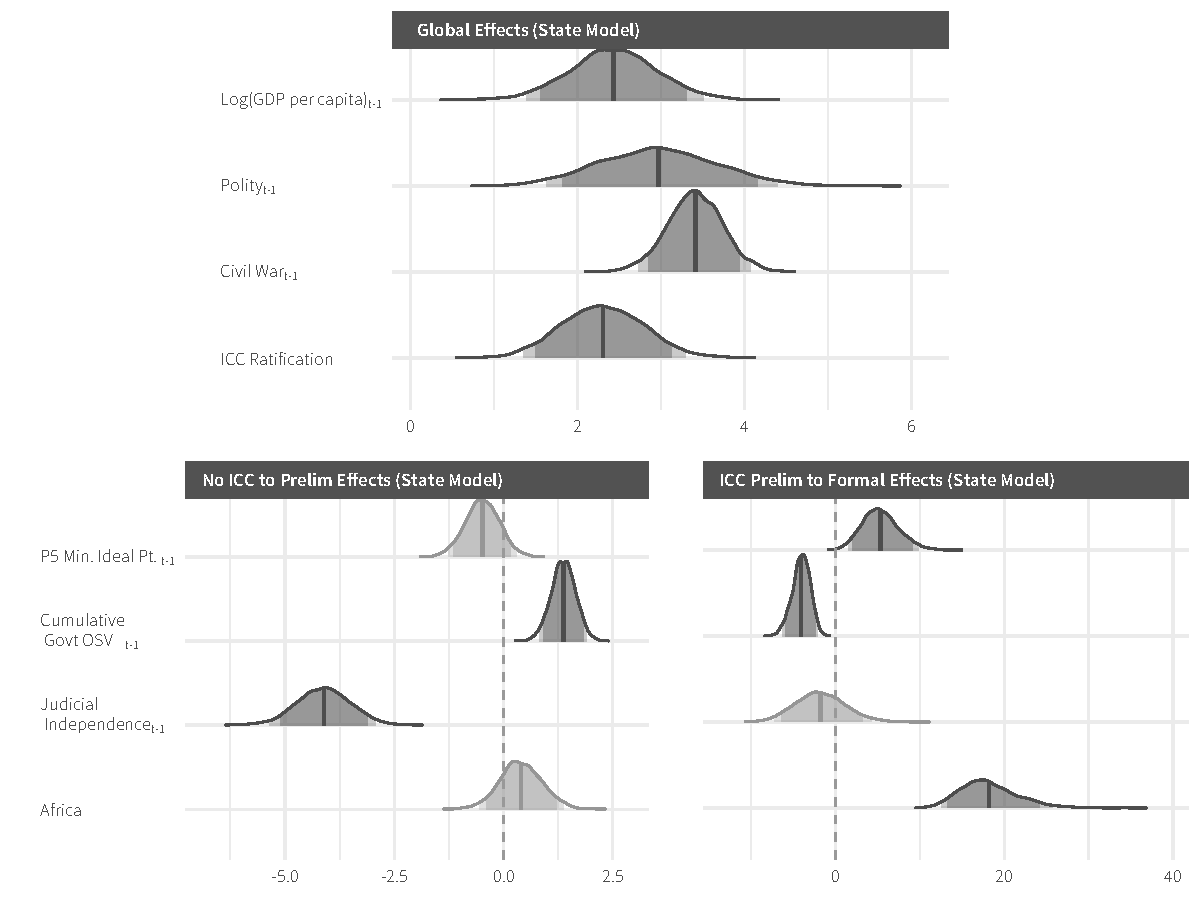
\includegraphics[width=1\textwidth]{stateCoefSumm.pdf}
    \caption{Parameter estimates from State-Focused ICC Transition model visualized through posterior distributions with median values designated by vertical line, lightly shaded portion indicating the 95\% credible interval, and darker shaded portion the 90\% credible interval.}
    \label{fig:stateModel}
\end{figure}

\begin{figure}
    \centering
    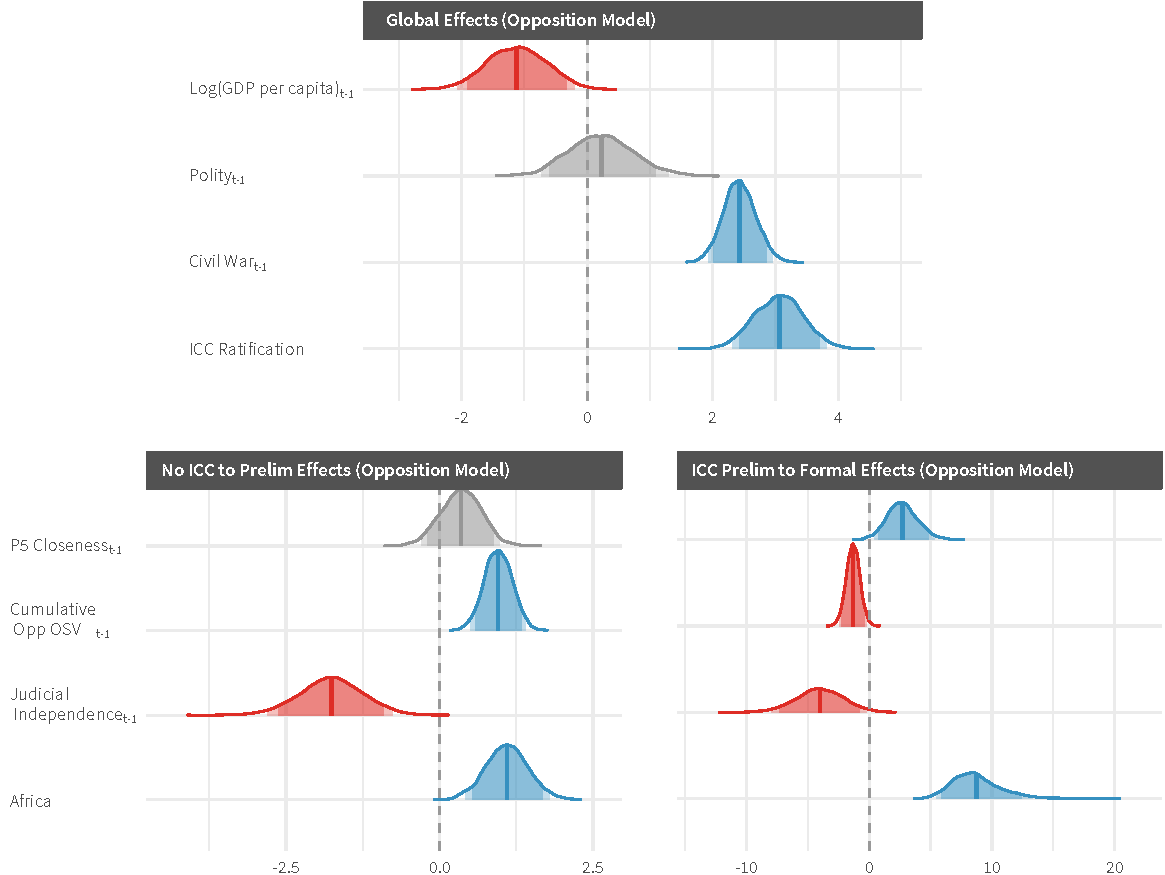
\includegraphics[width=1\textwidth]{rebelCoefSumm.pdf}
    \caption{Parameter estimates from Opposition-Focused ICC Transition model visualized through posterior distributions with median values designated by vertical line, lightly shaded portion indicating the 95\% credible interval, and darker shaded portion the 90\% credible interval.}
    \label{fig:rebelModel}
\end{figure}
% figure out a better way to depict results, since plots won't print in color - the grey vs blue vs red won't show up... right?

Figure \ref{fig:stateModel} presents the results for the transition to a \textit{government-targeted} preliminary examination and formal investigation. Figure \ref{fig:rebelModel} presents the results for \textit{opposition-targeted} preliminary examinations and formal investigations.
% add something here about what the figures present - standardized coefficient estimates with credible intervals? Something else? also add a sentence justifying standardized coefficients, and explain that they're useful for comparing size of effect across variables of interest.  I'm not sure what to say here - either Ben or SM can fill in.

Based on the logic of impartiality, we hypothesized that the OTP would be more likely to initiate a preliminary examination and advance to a formal investigation targeting a particular government when that government perpetrated more civilian targeting (H1), and that the OTP would be less likely to initiate examinations or advance to investigations against governments with more independent judiciaries (H2). The results in Figure \ref{fig:stateModel} demonstrate that the decision to initiate a preliminary examination (i.e. move from no ICC involvement to a preliminary examination) clearly follows the logic of impartiality. In line with H1, as the severity of government one-sided violence increases, the likelihood of the onset of a preliminary examination targeting that government also increases.  More substantively, the coefficient estimate for the OSV variable is 1.37, indicating that a one standard deviation increase in one-sided violence is associated with a 1.37 increase in the likelihood that the OTP initiates a preliminary examination against the government.
% i'm not clear on what units the 1.37 increase is.  a 1 standard deviation increase in OSV is associated with a 1.37 increase... what does this mean?  either add in % change info or take out the numbers altogether and just discuss how size of effect is larger/smaller than other key IVs (this goes for all similar comments below)

Similarly, in support of H2, increasing judicial independence reduces the likelihood that the OTP initiates a preliminary examination against the government. Thus, when considering the decision to initiate the first stage of ICC involvement against the government, the OTP's strategic decision-making does appear to be informed by the logic of impartiality. Interesting, the results suggest that this variable has a stronger substantive impact on OTP decision-making compared to the OSV measure. In particular, a one standard deviation increase in judicial independence is linked with a 4.12 decrease in the likelihood that the OTP starts a preliminary examination against the government. The judiciary variable also performs well compared to the other variables in the model; it has the largest substantive impact among the theoretical variables of interest and performs well against the global coefficients for the control variables.
% again unclear on the units for the size of effect 4.12 decrease

A similar picture emerges when considering the decision to initiate a preliminary examination targeting opposition actors. As Figure \ref{fig:rebelModel} demonstrates, increasing the level of one-sided violence perpetrated by opposition actors increases the likelihood that the OTP initiates a preliminary examination targeting the opposition, in line with H1. Specifically, we see that a one standard deviation increase in OSV is associated with a .96 increase in the likelihood that the OTP starts a preliminary examination against opposition actors.
% again question about units for the .96 increase

In line with the logic of impartiality, judicial independence again reduces the likelihood of the OTP initiating a preliminary examination in the opposition model.  Here, the coefficient estimate is -1.76, suggesting that a one standard deviation increase in the independent judiciary variable is associated with a 1.76 decrease in the likelihood of a preliminary examination targeting the opposition. Similar to the government model, the judiciary variable has the strongest substantive impact among the theoretical variables of interest.
% units for 1.76 decrease?

At the first stage, therefore, when the OTP must decide whether to initiate a preliminary examination, it appears that the logic of impartiality does influence her decision-making, whether crimes have been perpetrated by government or opposition actors. Furthermore, the result also suggest that complementarity, as proxied by an independent judiciary, has a strong impact on OTP decision-making, relative to the other theoretical variables of interest.

The OTP's incentive to adhere to the ICC's legal mandate, however, does not consistently extend to the decision to advance a situation to a formal investigation. While the logic of impartiality suggests that the OTP should prioritize the worst human rights abuses at both decision points, the results in Figure \ref{fig:stateModel} and Figure \ref{fig:rebelModel} indicate that the OTP is actually \textit{less} likely to advance from a preliminary examination to a formal investigation as abuses against civilian populations increase. While this negative effect seems surprising at first, we suspect that the OTP may be wary of advancing to an investigation in situations where the ability of the court's investigators to safely carry out their investigations and the security of witnesses may be compromised.\footnote{The deterrent effect of high OSV should be felt most at the second stage, when the OTP decides whether to initiate a formal investigation, as this stage requires a much greater OTP presence (i.e. investigators) on the ground.}

The effect of judicial independence is similarly weaker at the second stage. While more independent judiciaries reduce the likelihood of transition to formal investigations targeting opposition actors, as expected, judicial independence has no significant effect on the likelihood of moving from a preliminary examination to a formal investigation against government actors. %While more research is necessary to better understand the mixed results, it is possible that we observe a significant impact for judiciary only in the opposition model because governments may be more likely to prosecute members of the opposition than their own supporters to ward off a formal investigation.
%do you have any thought about why we find contradictory results.
% I'm not sure we want to make that point about why the effect doesn't hold in state model b/c it highlights that our measure is a pretty crappy proxy. I think its probably true that Judicial independence has no effect in the state model b/c it is probably associated with more trials against opposition than against state, and therefore OTP is still acting against states sometimes even when judiciary is independent.  but that just means our measure is bad. It suggests that the OTP could still be following the legal mandate, but we have no idea if that's true or not, since we don't directly measure complementarity.  We could just speculate more vaguely that more research is necessary to understand whether the null result is because the OTP's decision is less driven by complementarity in the second stage, or whether instead our measure needs further refinement. Not sure what the best strategy is.

Regarding the substantive impact in the opposition model, we see that a one standard deviation increase in judicial independence is associated with a 4.02 decrease in the likelihood that OTP moves to a formal investigation. Despite this significant result, it is nonetheless important to note that in the second stage,  we find no support for H1, and only mixed support for H2, suggesting that OTP decision-making is not primarily driven by the logic of impartiality in the second stage, when deciding whether to advance preliminary examinations to the formal investigation stage.

Unlike the logic of impartiality, the OTP's strategic incentives to consider P5 interests suggested that the OTP would target actors in states with weaker ties to the P5 when deciding whether to initiate a preliminary examination or advance to a formal investigation (H3). We again find mixed support for this argument. At the first stage, the OTP does not seem to be driven by incentives to prioritize P5 interests: distance from P5 states has no significant effect on the initiation of a preliminary examination in either the government (Figure \ref{fig:stateModel}) or opposition (Figure \ref{fig:rebelModel}) model. In other words, this result suggests that the OTP does not cater to powerful states' interests in an attempt to curry favor and increase their support for the court when deciding whether to open a preliminary examination targeting either government or opposition actors in a country.

At the second stage, on the other hand, P5 interests, as measured by ideal point distance, have a powerful effect on the OTP's decision-making. As demonstrated in Figures \ref{fig:stateModel} and \ref{fig:rebelModel}, the OTP is significantly more likely to advance a preliminary examination to the formal investigation stage against governments and opposition actors in states with weaker ties to powerful states (i.e. the P5). Substantively, we see that a one standard deviation increase in P5 ideal point distance is associated with a 5.5 and 5 increase in the onset of formal investigations in the government and opposition models, respectively.
% again, clarify unit of 5.5 and 5 increase.

The results for Africa are largely similar to those for the ideal point distance measure, as they vary across stages of ICC involvement. In the preliminary examination stage, Africa is only statistically significant in the opposition model. In particular, a one standard deviation increase is associated with a 1.10 increase in the likelihood that the OTP initiates a preliminary examination against opposition actors. Interestingly, the substantive impact of this variable is smaller than the other statistically significant variables and the the control variables. Thus, the relatively small substantive effect along with insignificant result in the government model raises important questions regarding the conventional wisdom of the so-called African bias, which claims that the OTP is always more likely to target Africans because of African states' relatively smaller geo-strategic importance to powerful states.
% again, clarify unit for the 1.1 increase for Africa in opposition model
% is the effect of Africa really smaller than OSV?  it doesn't look that way in the figure, but i might be wrong. can we say effect is smaller than the impartiality variables specifically, instead of saying "other significant variables"?  Again i'm also wary of comapring to the controls since those are global coefficients.

On the other hand, we find that Africa is associated with a higher probability of formal examinations in both the government and opposition models. Not surprisingly, this variable produces the largest substantive effect in the second stage, as the coefficient estimates are 18.19 and 8.74 in the government and opposition models, respectively. These results are also in line with the findings from the ideal point distance measure for P5 interests. Taken together, the results for Africa across the two stages of the two models reinforces the conclusion that the OTP's decision-making is affected by the interests of powerful states primarily at the second decision point, when deciding whether to advance a preliminary examination to the formal investigation stage. The results for Africa also speak to the claim that the OTP is biased against Africa: the OTP's tendency to favor African targets appears to be largely limited to the formal investigation stage.

Turning briefly to control variables, we find that they behave largely as expected across the models. As a reminder, we only assess the global effects of the controls due to sparse data. As expected, in both the government and opposition models, both civil war and ICC ratification are significantly associated with a higher probability of ICC involvement. The results for polity, on the other hand, do not match expectations: polity is insignificant in the opposition model, and is positive and significant in the government model. This unexpected positive result is likely driven by high-profile examinations of government actors in strongly democratic states, including the US, UK, and Israel. We also see mixed results for GDP per capita; the measure is positive and significant in the government model, while it is negative and significant in the opposition model. While this result requires more research, it is not entirely surprising, given that we anticipated that economic development could affect OTP involvement in different ways with contradictory effects.
% Ben, is what I said about democracy result OK?

% add paragraph here about model fit and comparison to ologit, selection model, etc. demonstrate that our model produces better and different results (assuming that's true).  we probably also need to think about selection type models, and why we don't use those (or how our results are better than if we used those, since the selection process is kind of obvious here and IR people will think that's an obvious modeling strategy, moreso than ologit probably)
